%%
%% Beuth Hochschule für Technik --  
%%
%% Kapitel 4 - 
%%
%%	

\newpage
[Perkowski]
\section{Messtechnische Identifikation des Störverhaltens der Strecke}
Da das Verhalten der Störübertragungsfunktion zu ermitteln ist, kann wie im Kapitel 3 durchgeführt werden. Die Strecke wird erst in den Arbeitspunkt erregt und dann die Störgröße mit einem Schalter an der Hardware zugeschaltet. Wir haben die Störmessung aufgezeichnet \textit{(stoer\_err.mat)}.

\begin{figure}[h]
	\begin{center}
		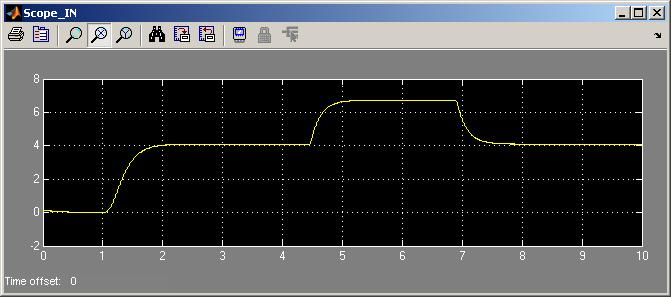
\includegraphics[scale=0.5]{stoerung.jpg}
		\caption{Strecke mit Störung}
       \label{stoer}
	\end{center} 
\end{figure}

Nachdem wir die gemessene Sprungantwort betrachten, sind wir aufgrund des typischen Verhaltens ausgegangen, dass es sich um PT1-System handelt. 
Da mit Hilfe des Tools \textit{sys\_id} die Zeitachse der Störung eingegrenzt werden kann, kann an dieser Stelle die Identifikation der Störstrecke durchgeführt werden. Das Ergebnis kann im folgenden Bild nachvollzogen werden.

Die ermittelte Störungsfunktion:

\begin{center}
$ G(s)_{stoer} = \dfrac{2,6424}{1 + 0,16207} $
\end{center}

\begin{figure}[h]
	\begin{center}
		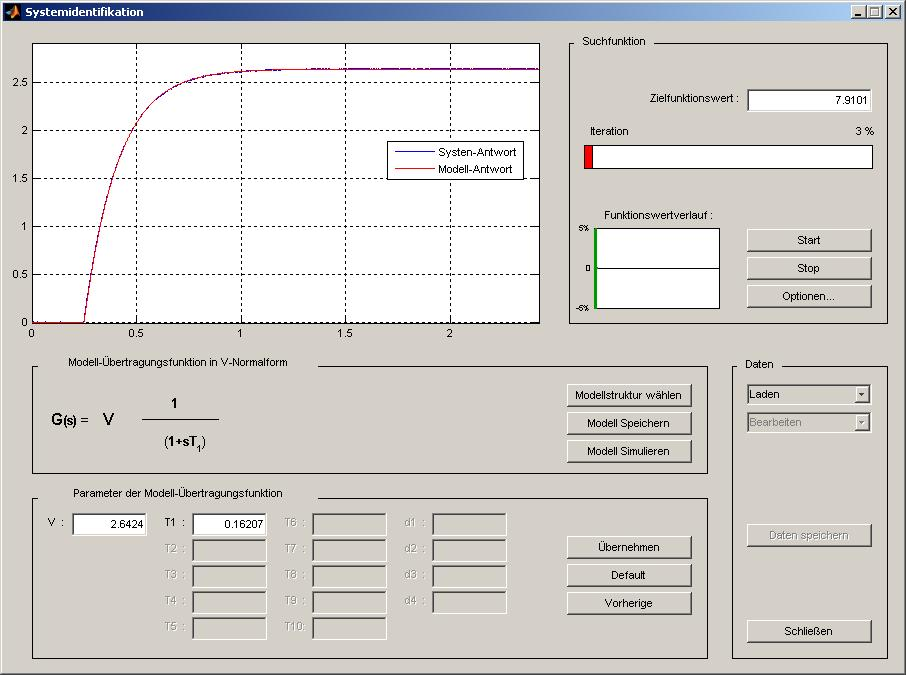
\includegraphics[scale=0.5]{stoerung_1_uebfkt.jpg}
		\caption{erster Ausschnitt Übertraungsfunktion mit Störung}
       \label{stoerfkt1}
	\end{center} 
\end{figure}

\begin{figure}[h]
	\begin{center}
		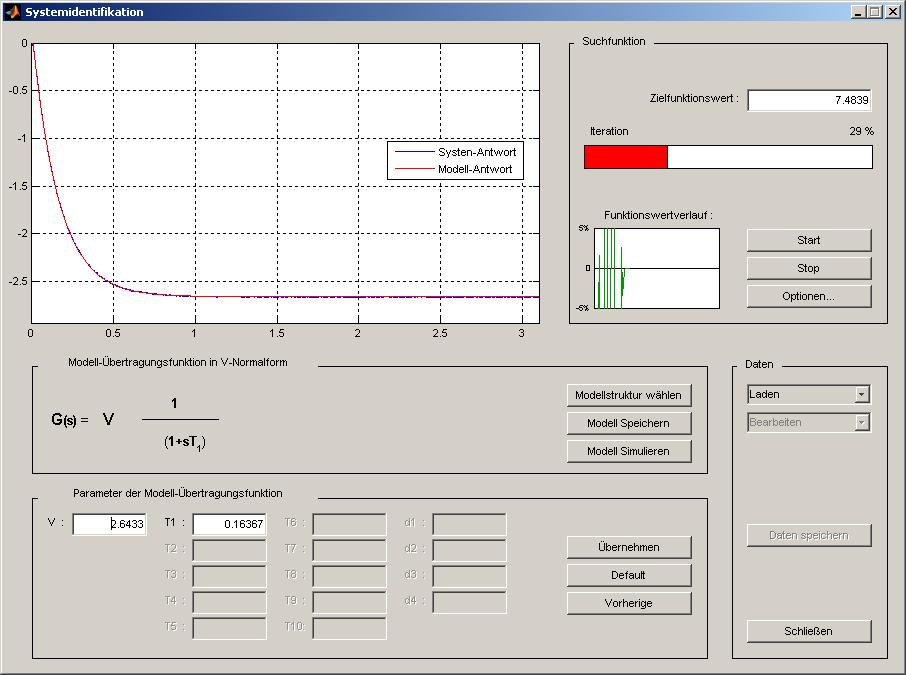
\includegraphics[scale=0.5]{stoerung_2_uebfkt.jpg}
		\caption{zweiter Ausschnitt Übertraungsfunktion mit Störung}
       \label{stoerfkt2}
	\end{center} 
\end{figure}

